\documentclass{article}
\usepackage{graphicx} % Required for inserting images
\usepackage{amsmath}
\usepackage{siunitx}

\title{Interactive EM Math}
\author{Benjamin Cates}
\date{February 2023}

\begin{document}

\maketitle
\section{Symbols}
For the remainder of this text $\vec{p}$ will be the point that the test charge is placed at and the distance from a point charge is $r$. Each object has a center $\vec{c}$ and rotation $\theta$, or it's position is defined in a unique way in it's section. Finally, each has either a charge $Q$, linear charge density $\lambda$, or an area charge density $\sigma$. The symbol $K$ will be used as Coloumb's constant. Definitionally, voltage is $V=\frac{KQ}{r}$ and electric field is $\vec{E}=\frac{KQ}{r^2}\hat{r}$ where $\hat{r}$ points away from the source. It also follows that $\vec{E} = -\nabla V$.

\section{Point charges}
\subsection{Voltage}
The voltage of a point charge is definitionally defined as
\begin{equation}
    V=\frac{KQ}{\lVert \vec{p}-\vec{c}\rVert }
\end{equation}
\subsection{Electric Field}
The electric field of a point charge is also definitionally defined.
The field of a point charge is simply $\vec{E} = \frac{KQ}{r^2}\frac{\vec{r}}{r}$.
\begin{equation}
\frac{KQ}{\lVert \vec{p}-\vec{c} \rVert^3}(\vec{p}-\vec{c})
\end{equation}
\subsection{Torque}
Point charges have no radius, so they have no moment of inertia and also have no torque put upon them.
\section{Infinite Plane}
\subsection{Voltage}
The integral of $\frac{KQ}{r}$ over the surface of an infinite plane is infinity, we will use the path integral of integral of $\vec{E} = 2\pi K\sigma$, which is already known. The electric field is obviously constant, so moving a distance $d$ away from the plane will decrease the potential energy by $2\pi K \sigma d$. Adding on a constant accounts for the possible infinity that results from the other method. In reality, this constant could be a reasonable number because all voltage is relative. Anyway, we still have to adjust to fit the confines of the program, including "center" of the plane (which will be a reference for a point on the plane).

From vector math, we know the distance from a plane is $d= \vec{n}\cdot\vec{P_0P}$, so the distance in our program is $d=\langle-\cos{\theta},\sin{\theta}\rangle\cdot(\vec{p}-\vec{c})$. Therefore, the final formula is shown below
\begin{equation}
    V(\vec{p}) = C - 2\pi K\sigma \langle-\cos{\theta},\sin{\theta}\rangle\cdot(\vec{p}-\vec{c})
\end{equation}

\subsection{Electric Field}
The field of an infinite plane is well-known to be $2\pi K\sigma \hat{r}$. In our program, we have to figure out how to determine the $\hat{r}$, but it's obviously either equal to $\vec{n}$ or $-\vec{n}$. We used the sign function with the dot product of the normal and a vector from the plane to the point, which will be positive if they face the same direction and negative if they face the opposite. The final formula is
\begin{equation}
    \vec{E}(\vec{p}) = 2\pi K\sigma\vec{n}\ \text{sgn}((\vec{p}-\vec{c})\cdot\vec{n})\ \text{where}\ \vec{n}=\langle-\sin(\theta),\cos(\theta)\rangle
\end{equation}

\subsection{Torque}
Planes are infinite so their moment of inertia is infinity and torque on them has no effect.

\section{Finite Line}
For the finite line, it also has the property $w$ which is half of the width. We will start by assuming that the line's center is $\vec{0}$ and the rotation is zero, so the line will be along the x-axis.\\
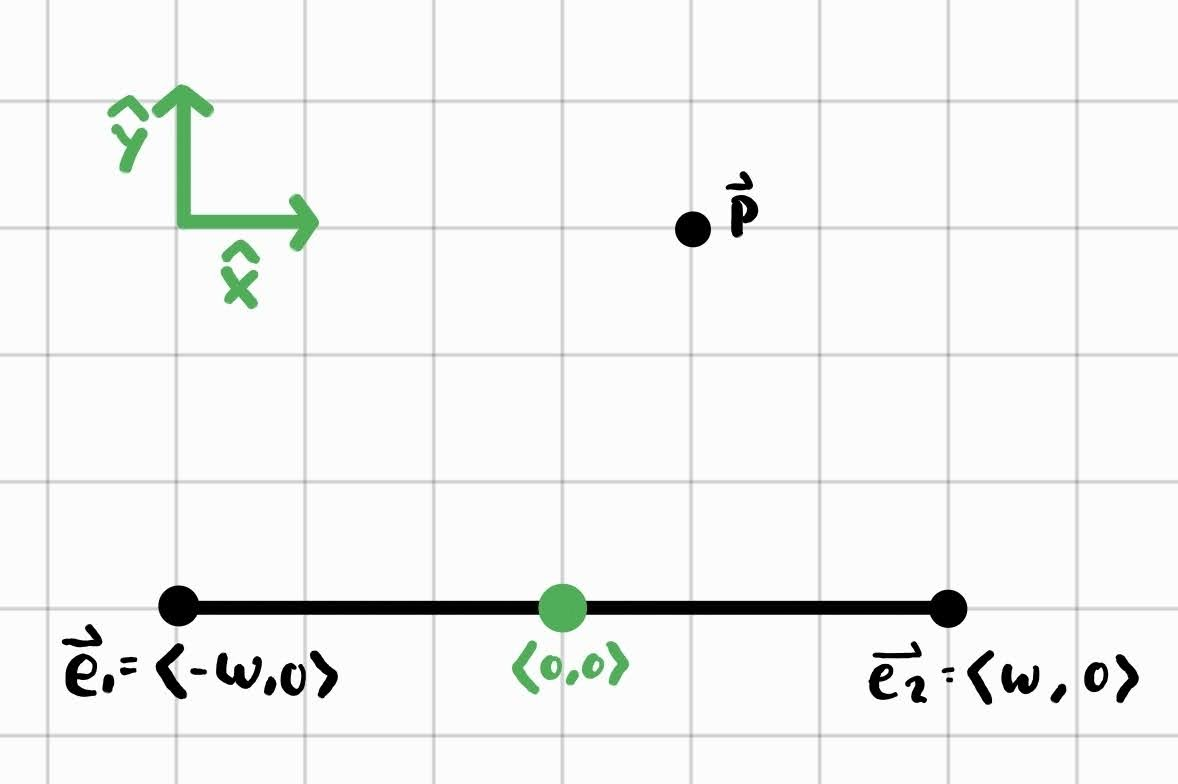
\includegraphics[scale=0.25]{finite_line_setup.jpg}
\subsection{Voltage}
\begin{align*}
    V &= \int_{-w}^w \frac{K \lambda dx}{\sqrt{(p_x-x)^2+p_y^2}} \\
    &\text{let}\ x=p_x-x \\
    &dx = -dx \\
    &= -K\lambda\int_{p_x+w}^{p_x-w} \frac{dx}{\sqrt{x^2+y^2}} \\
    &= K\lambda\int_{p_x-w}^{p_x+w} \frac{dx}{\sqrt{x^2+y^2}} \\
    &= K\lambda \ln{\left(\sqrt{x^2+y^2}+x\right)} |_{p_x-w}^{p_x+w} \\
    &= K\lambda \ln{\left|\frac{\sqrt{(p_x+w)^2+p_y^2}+p_x+w}{\sqrt{(p_x-w)^2+p_y^2}+p_x-w}\right|}
\end{align*}
Define $\vec{e_1} = \vec{c} - w\langle\cos(\theta),\sin(\theta)\rangle$ and $\vec{e_2} = \vec{c} + w\langle\cos(\theta),\sin(\theta)\rangle$ to be the endpoints of the line.
\begin{align*}
    V &= K\lambda \ln \left(\frac{\lVert \vec{p}-\vec{e_1}\rVert+p_x+w}{\lVert \vec{p}-\vec{e_2}\rVert+p_x-w}\right)
\end{align*}
In order to adjust for the angle and center of the line, we will replace $p_x$ with the linear transformation $\vec{p} \cdot \langle\cos(\theta),sin(\theta)\rangle$ and rename it as $g$.
\begin{equation}
    V(\vec{p}) = K\lambda \ln \left( \frac{\lVert\vec{p}-\vec{e_1}\rVert+g+w}{\lVert\vec{p}-\vec{e_2}\rVert+g-w} \right)
\end{equation}
\subsection{Electric Field}
WRITE HERE
\subsection{Torque}
The moment of inertia of a finite line about the center is well known to be $\frac{1}{12}ML^2$.



\section{Conductors}
For this entire program, we are working in 2d, so there is no obvious way to have conductors. We could either have sheets of conductor that
\subsection{Setup}
The goal of a conductor in this program is to have a constant voltage along the edge and a constant voltage on the inside of a conductor. We made a generic class that only takes in the location of points of charge and test points where the voltage should be measured. In order to not mess with the dimensionality, the point charges are actually line charges that extend a couple of meters in either direction because an infinitely thin conductor has no effect, and a plate conductor facing the viewer would not look as cool.
\subsection{Linear Algebra}
The following is the system of linear equations that we have to solve, or at least get the closest possible answers to:
\begin{alignat*}{7}
    &\ \ Q_1&+&\ \ Q_2 &+&\ \ Q_3 &+& \ldots &+&\ \ Q_n &&= Q_{net}\\
    &\frac{KQ_1}{r_{11}} &+& \frac{KQ_2}{r_{12}} &+& \frac{KQ_3}{r_{13}} &+&\ldots &+& \frac{KQ_n}{r_{1n}} &&= C-V_1\\
    &\frac{KQ_1}{r_{21}} &+& \frac{KQ_2}{r_{22}} &+& \frac{KQ_3}{r_{23}} &+&\ldots &+& \frac{KQ_n}{r_{2n}} &&= C-V_2\\
    &\frac{KQ_1}{r_{31}} &+& \frac{KQ_2}{r_{32}} &+& \frac{KQ_3}{r_{13}} &+&\ldots &+& \frac{KQ_n}{r_{3n}} &&= C-V_3\\
    &\ \ \vdots& & \ \ \vdots & & \ \ \vdots & & \ddots & & &&\ \ \vdots\\
    &\frac{KQ_1}{r_{m1}} &+& \frac{KQ_2}{r_{m2}} &+& \frac{KQ_3}{r_{m3}} &+&\ldots &+& \frac{KQ_n}{r_{mn}} &&= C-V_m\\
\end{alignat*}
Where $Q_i$ is the ith charge point, $r_ij$ is the distance between the ith test point and the jth charge point, $C$ is the voltage of the conductor, and $V_j$ is the external voltage at the jth test point.
If we subtract $C$ from both sides, this leads to a $m+1$ by $n+1$ matrix equation of the form
\begin{equation*}
\begin{bmatrix}
1 & 1 & 1 &\ldots& 1 & 0\\
\frac{K}{r_{11}} & \frac{K}{r_{12}} & \frac{K}{r_{13}} &\ldots& \frac{K}{r_{1n}} & 1\\
\frac{K}{r_{21}} & \frac{K}{r_{22}} & \frac{K}{r_{23}} &\ldots& \frac{K}{r_{2n}} & 1\\
\frac{K}{r_{31}} & \frac{K}{r_{32}} & \frac{K}{r_{33}} &\ldots& \frac{K}{r_{3n}} & 1\\
\vdots &\vdots & \vdots &\ddots& \vdots & \vdots\\
\frac{K}{r_{m1}} & \frac{K}{r_{m2}} & \frac{K}{r_{m3}} &\ldots& \frac{K}{r_{mn}} & 1
\end{bmatrix}
\begin{bmatrix}
    Q_1\\
    Q_2\\
    Q_3\\
    \vdots\\
    Q_n\\
    -C\\
\end{bmatrix}
=
\begin{bmatrix}
    Q_{net}\\
    -V_1\\
    -V_2\\
    -V_3\\
    \vdots\\
    -V_n\\
\end{bmatrix}
\end{equation*}
Which we will reduce to write as $A\vec{Q} = -\vec{V}$. Solving this linear system of equations is impossible to do exactly because there might be more test points than charge points, however, we can solve for the least squares solution which is governed by the equation $\vec{V} = (A^TA)^{-1}A^T\vec{Q}$. Since the matrix part is constant for each shape of object, it can be calculated once at the object construction and the charge at each point can be computed with a simple vector transformation.
\subsection{3d Correction}
Since 2d conductors do not actually exist, we are treating the conductor as if it is extruded a couple of units in the z direction. This would mean that each point charge would behave similar to a line charge, so we used the voltage and field caused by a line charge that was mentioned earlier. However, this approximation did not come out well because the charge density tapers off near the ends. We will assume for simplicity that the charge density changes at a linear rate. Instead of having a $Q$ for each line, we now have $\lambda_1$ and $\lambda_2$ for the center and the tip respectively. Since the entire simulation is symmetrical across the z-axis, we will just mirror every thing by multiplying or dividing by 2. We will also assume that the conductor has a variable height $h$. Let's start with the voltage on the $z=0$ plane.
\begin{align*}
    V &= \frac{Q}{r}\\
    V &= \int_0^h \frac{(\lambda_1 + \frac{z}{h}(\lambda_2-\lambda_1)) dz}{\sqrt{z^2+r^2}}\\
    &= \lambda_1\int_0^h \frac{1}{\sqrt{z^2+r^2}} + (\lambda_2-\lambda_1)\int_0^h \frac{z}{\sqrt{z^2+r^2}}\\
    &= \lambda_1\ln\left(\frac{h+\sqrt{h^2+r^2}}{r}\right)+(\lambda_2-\lambda_1)(\sqrt{h^2+r^2}-r)\\
\end{align*}
We also need to add another test point at a different location outside of the flat plane. So we'll add a test point next to the position of $\lambda_2$, which will also require us to account for the mirroring because the mirrored half is further away. So the density will vary from $\lambda_2$ to $\lambda_1$ over the distance $0$ to $h$, and then it will vary from $\lambda_1$ to $\lambda_2$ over the interval $h$ to $2h$. We will define $d_h = \sqrt{h^2+r^2}$, $d_{2h} = \sqrt{(2h)^2+r^2}$, and $\Delta\lambda = \lambda_2-\lambda_1$.
\begin{align*}
    V &= \int_0^h \frac{\lambda_2 - \frac{z}{h}\Delta\lambda dz}{\sqrt{z^2+r^2}} + \int_h^{2h} \frac{\frac{z-h}{h}\lambda_2 + \frac{2h-z}{h}\lambda_1}{\sqrt{z^2+r^2}}dz\\
    V &= \lambda_2\ln\left(\frac{h+d_h}{r}\right)-\Delta\lambda(d_h-r)+\frac{\Delta\lambda}{h}(d_{2h}-d_h) + (\lambda_1-\Delta\lambda)\ln\left(\frac{2h+d_{2h}}{h+d_h}\right)
\end{align*}
Now we can replace the $\frac{KQ}{r}$ in the matrix with these formulas. $\lambda_1$ and $\lambda_2$ will be treated as "charge" points, and the test points will be doubled in the z direction.


\section{Calculating Inertia}
The parallel axis theorem states that $I = I_C + Md^2$. Where I is the moment of inertia about an arbitrary point, $I_C$ is the moment of inertia about the center, $M$ is the mass of the object, and $d$ is the distance between the arbitrary point and the center of mass of the object.

\section{Algorithms}
include here the algorithm for getting force between each element

\section{Magnetic Field}
For moving charges, the formula for the electric field is
\begin{equation}
    \vec{B} = \frac{\mu _0}{4\pi}\frac{q\vec{v}\times\hat{r}}{r^2}
\end{equation}
Where $\mu _0 = 1.257\times 10^{-6} \si{\frac{N}{A^2}}$. For moving charges, the strength of this force is weak because $\mu _0$ is a small number. We will not implement the magnetic field in the program because it is only significant for currents. For two moving charges, the ratio between magnetic force and electric force is $\frac{ F_{\vec{B}} }{F_{\vec{E}} } = \frac{v^2}{c^2}$, so for $v \ll c $, the magnetic force is nothing compared to the electric force.
\end{document}
